\chapter{The $\alpha$-shapes approach}\label{chap:boundaries_alpha}
In the previous chapter we presented a new ray tracing approach based on PS. We explained that, in order to compute the target intensity, it is necessary to know the boundaries of the regions in target PS with positive luminance. Ray tracing in PS requires tracing only the rays close to these boundaries. The rays traced can be seen as a point cloud in PS. To detect the shape formed by those rays, the $\alpha$-shapes approach is employed \cite{portegies2013fast}.\\ \indent
Methods based on $\alpha$-shapes are widely used to reconstruct an unknown shape formed by a set of finite data points \cite{guo1997surface}. $\alpha$-shapes is a very powerful tool to construct the shape of a point cloud. As the parameter $\alpha$ varies, we can obtain different $\alpha$-shapes from the point set itself to the convex
hull \cite{xu2003automatic}. The disadvantage of such method is that it can be very hard to choose the appropriate value of the parameter $\alpha$ and, in most cases it can be selected only by trial-and-error.\\ \indent
We developed a technique based on $\alpha$-shapes that gives a criterion to determine the value of the parameter $\alpha$, for which the boundaries are approximated well \cite{filosa2015new}.\\ \indent This chapter is organized as follows. An overview of the-state-of-the-art about $\alpha$-shape methods is provided in Section \ref{sec:alpha-shapes}; the technique used for computing the $\alpha$ value is explained in Section \ref{sec:Tir_alpha}; the results for two different kind of total internal reflection (TIR)-collimators are given in Section \ref{sec:results-Tir-alpha}. Discussions and conclusions are provided in the last paragraph of this chapter.
\section{$\alpha$-shapes theory}\label{sec:alpha-shapes}
Given a finite set $\mbox{\insieme{U}} = \{\point{u}_1, \cdots, \point{u}_N\}\subset \mathbb{R}^2$ of points, $\alpha$-shapes are geometrical objects that give us an approximation of the shape formed by the point cloud. For now we do not further specify the notion of shape. A more precise definition will be provided later.\\ \indent
Before giving a formal definition, we explain an intuitive and nice interpretation of $\alpha$-shapes \cite{lucieer2004alpha}. 
Let us think of a stracciatella ice-cream\footnote{Stracciatella ice cream is made with milk-based ice-cream and fine pieces of chocolate \cite{Wiki3}.}. If we desire to know the shape formed by the chocolate pieces we can start eating the ice cream using a spoon with a spherical scoop and try not to remove any piece of chocolate. 
We will obtain a shape formed by arcs and points. % (see Figure \ref{fig:shape2d} for the two-dimensional case).
%\begin{figure}[t]\label{fig:shape2d}
%\begin{center} 
%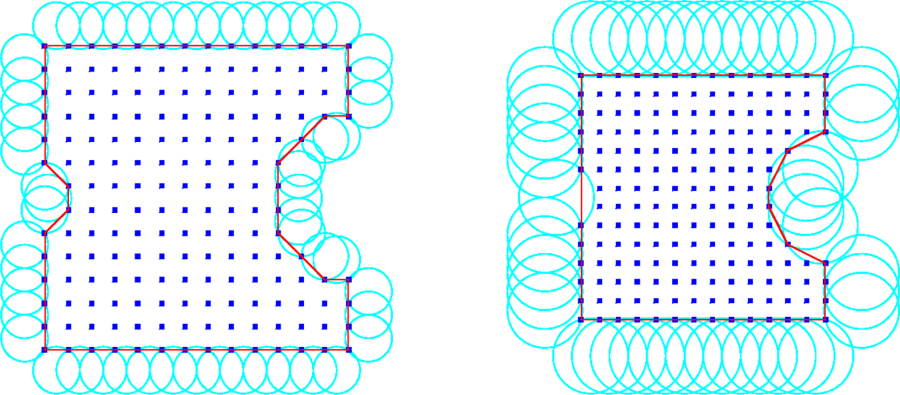
\includegraphics[width=\textwidth]{alpha_shape2D}
%\label{fig:shape}
%\caption{\textbf{Construction of $\alpha$-shapes.} The boundary of the shape (red line) formed by a set of points (blue dots) in $\mathbb{R}^2$ is detected for $\alpha = 1$ (left) and for $\alpha=2$ (right) \cite{sabel2017application}.}
%\label{fig:shape2d}
%\end{center}
%\end{figure}
Straightening the arcs to line segments we obtain broken lines which constitute the boundary of the so-called $\alpha$-shape of the point set $\mbox{\insieme{U}}$. 
A very small spoon will allow us to eat the entire ice cream without eating any piece of chocolate, while with a larger spoon we are not able to eat any chunk of the ice cream without chocolate pieces. In this example, the chocolates pieces are the points of set $\mbox{\insieme{U}}$ and, the parameter $\alpha$ determines the radius of the carving spoon (the spherical spoon in two-dimension is simply a circle).\\ \indent 
The formal definition of $\alpha$-shape was first given by Edelsbrunner, Kirkpatrick and Seidel in 1983 \cite{edelsbrunner1983shape}. They describe $\alpha$-shape as a generalization of the convex hull of a finite set of points in the plane. Let $\alpha$ be a non negative number $0\leq\alpha<\infty$. 
If $\alpha = 0$ the shape degenerates to the point set $\mbox{\insieme{U}}$. On the other hand, when $\alpha\rightarrow\infty$ the $\alpha$-shape is simply the convex hull of \insieme{U}. If $0<\alpha<\infty$ the $\alpha$-shape is a polygon of \insieme{U} \cite{edelsbrunner1994three}. The construction of the $\alpha$-shape is closely related to the Delaunay triangulation of \insieme{U} \cite{mucke1993shapes}. Therefore, a formal definition of triangulation and Delanauy triangulation is now required. \\ \indent
Given a set $\mbox{\insieme{U}}$ of points not all aligned, let us consider the set \insieme{E} of all the straight-line segments whose endpoints are in \insieme{U}. 
A triangulation \insieme{T} of $\mbox{\insieme{U}}$ is the subset of \insieme{E} with the maximum number of segments such that all the line segments of \insieme{T} intersect only at their endpoints \cite{lloyd1977triangulations}. 
\\ \indent Before giving a more formal definition of triangulation, let us define a partition of a set $\mbox{\insieme{X}}\subset \mathbb{R}^2$ as a collection of the subsets which divide \insieme{X} into non-overlapping regions so that any point in \insieme{X} is located in only one region. 
\begin{definition} \indent Let $\mbox{\insieme{P}}\subset \mathbb{R}^2$ be the convex hull of $\mbox{\insieme{U}}$ and $\mbox{\insieme{T}} = \{\mbox{\insieme{T}}_1, \cdots, \mbox{\insieme{T}}_\variabile{h}\}$ be a partition of $\mbox{\insieme{P}}$ into closed triangles, that is triangles that include their edges. Suppose that the following properties hold:
\begin{itemize}
\item[a)] $\mbox{\insieme{P}} = \bigcup_{\variabile{i} = 1}^{\variabile{h}}\mbox{\insieme{T}}_\variabile{i}$,
\item[b)] $\forall \mbox{ \insieme{T}}_\variabile{i}, \mbox{\insieme{T}}_\variabile{j} \in \mbox{\insieme{T}}$, $\mbox{\insieme{T}}_\variabile{i} \neq \mbox{\insieme{T}}_\variabile{j}$, and 
\begin{equation*}
\textrm{int}(\mbox{\insieme{T}}_\variabile{i})\cap \textrm{int}(\mbox{\insieme{T}}_\variabile{j}) = \emptyset,
\end{equation*}
where $\textrm{int}(\mbox{\insieme{T}}) = \mbox{\insieme{T}}-\partial \mbox{\insieme{T}}$,
\end{itemize}
then $\mbox{\insieme{T}}$ is called a \textit{triangulation} of $\mbox{\insieme{P}}$ \cite{Numericalmethods}.
\end{definition}
The Delaunay triangulation $\mbox{\insieme{T}}^{\prime}$ of the point set \insieme{U} has the property that the circumcircle of any triangle of $\mbox{\insieme{T}}^{\prime}$ does not contain any point of \insieme{U}. This is called the Delaunay property. A very commonly used algorithm to construct such triangulation is the following.\\ \indent 
$\mbox{\insieme{T}}^\prime$ is constructed by modifying a general triangulation \insieme{T} such that every point satisfies the Delaunay property. 
Therefore, every triangle that does not satisfy such property is flipped such that the new edge is part of the triangulation, see Figure \ref{fig:Delaunay}. 
Given, for example, an arbitrary triangulation \insieme{T} in two-dimensions, for each edge $\overline{\point{ab}}$ in \insieme{T} which is not on the boundary of the convex hull the two triangles 
$\Delta_{\point{abc}}$ and $\Delta_{\point{abd}}$ with the common edge $\overline{\point{ab}}$ are identified. Then, if either the circumcircle of triangle $\Delta_{\point{abc}}$ contains point \point{d} or the circumcircle of triangle $\Delta_{\point{abd}}$ contains point \point{c}, the edge $\overline{\point{ab}}$ cannot be included in the Delaunay triangulation and, therefore, $\overline{\point{ab}}$ is replaced by the edge $\overline{\point{cd}}$ such that the triangles $\Delta_{\point{acd}}$ and $\Delta_{\point{bcd}}$ are constructed. The new edge $\overline{\point{cd}}$ locally satisfies the Delaunay property and the triangles $\Delta_{\point{acd}}$ and  $\Delta_{\point{bcd}}$ are added to the Delaunay triangulation $\mbox{\insieme{T}}^\prime$.  
\begin{figure}[t]\label{fig:Delaunay}
\begin{subfigure}[t]{0.48\textwidth}
\centering
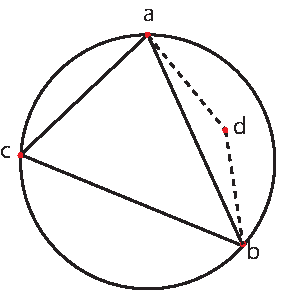
\includegraphics[]{triangle_alpha_shapes}
\label{fig:shape}
\caption{\textbf{Not acceptable triangle.} The point \point{d} is inside the circle circumscribing the triangle $\Delta_{\point{abc}}$, therefore the edge $\overline{\point{ab}}$ cannot be included in the Delaunay triangulation.}
\end{subfigure}
\hfill
\begin{subfigure}[t]{0.48\textwidth}
\centering
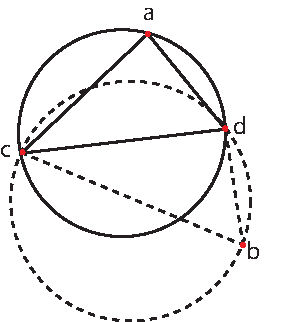
\includegraphics[]{triangle_alpha_shapes_flipped}
\caption{\textbf{Acceptable triangle.} The flipped triangle $\Delta_{\point{acd}}$ satisfies the Delaunay property, thus it is included in the Delaunay triangulation.}
\end{subfigure}
\caption{Construction of the Delaunay triangulation in 2D.}
\label{fig:Delaunay}
\end{figure}
\\ \indent Several other algorithms have been developed to construct a Delaunay triangulation, see for example \cite{lee1980two, renka1997algorithm}.
 Given a point set $\mbox{\insieme{U}}$ and a triangulation \insieme{T}, it can be proved that the corresponding Delaunay triangulation $\mbox{\insieme{T}}^\prime$ is unique. Moreover, it maximize the largest minimum angle among all possible triangulations of a point set $\mbox{\insieme{U}}$ \cite{press2007numerical}.
\\ \indent Alternatively, the Delaunay triangulation can be constructed as the dual of the Voronoi diagram \cite{fortune1992voronoi}. Let $\mbox{\insieme{X}}\subset\mathbb{R}^2$ be a metric space endowed with the Euclidean distance $d(\point{x}, \point{y})$ for $\point{x}, \point{y}\in \mbox{\insieme{X}}$. For \textit{almost}\footnote{Note the importance of the word \textit{almost}. Some points can have the same distance with two or more points of $\mbox{\insieme{U}}$.} every point $\point{x}\in \mathbb{R}^2$, there is a unique point that is the closest point to $\point{x}$. The Voronoi cell of a point $\point{u}_\variabile{i}\in \mbox{\insieme{U}}$ contains all points in $\mathbb{R}^2$ that are closest to $\point{u}_{\variabile{i}}$, see Figure \ref{fig:Voronoi}. The Voronoi diagram of $\mbox{\insieme{U}}\subset \mathbb{R}^2$ is defined as the set of all Voronoi cells \cite{cazals2005conformal}. A more formal definition of the Voronoi diagram is given in the following.
\begin{defn}
Let $\mbox{\insieme{U}}=\{\point{u}_1,\cdots,\point{u}_N\}$ be a set of points in $\mathbb{R}^2$. The Voronoi cell $\mbox{\insieme{V}}_\variabile{i}$ associated to point $\point{u}_\variabile{i}$ is defined as:
\begin{equation}
\mbox{\insieme{V}}_\variabile{i}=\{\point{x}\in \mathbb{R}^2\; | \;|\point{x}-\point{u}_\variabile{i}|<|\point{x}-\point{u}_\variabile{j}| \quad \forall \variabile{j}\neq \variabile{i} \}.
\end{equation}
The Voronoi diagram $\mbox{\insieme{V}}$ is defined as 
\begin{equation}
\mbox{\insieme{V}} = \bigcup_{\variabile{i}=1}^N \mbox{\insieme{V}}_\variabile{i}
\end{equation}
 where $\mbox{\insieme{V}}_{\variabile{i}}\cap \mbox{\insieme{V}}_{\variabile{j}}= \emptyset$ for $\variabile{i}\neq\variabile{j}$.
\end{defn}
For the definition of Voronoi diagram in higher dimensions see \cite{brown1979voronoi}.
\begin{figure}[t]
\centering
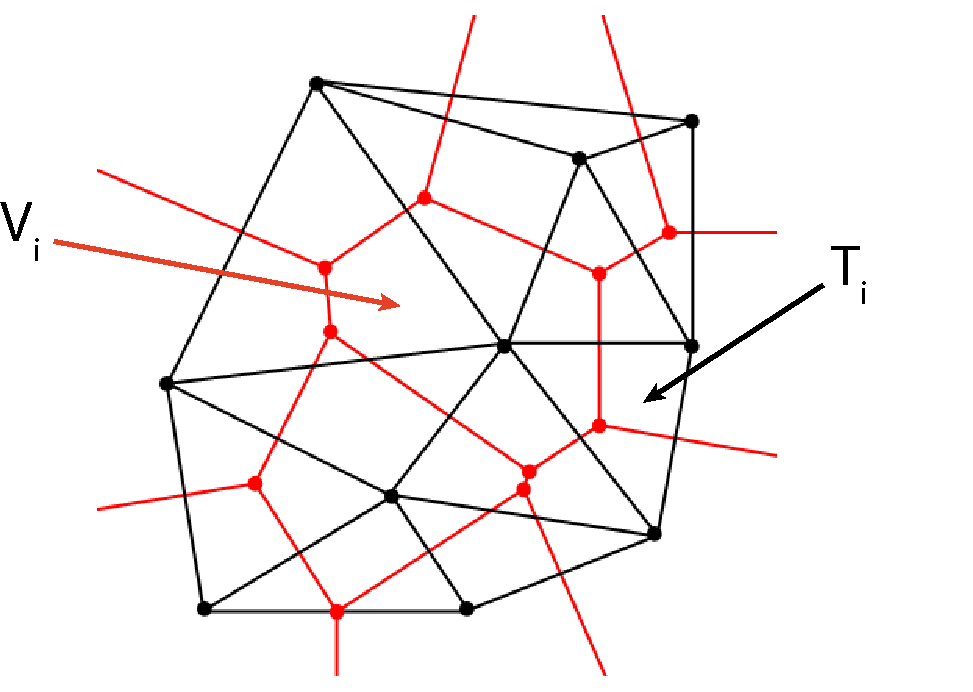
\includegraphics[width = 0.7 \textwidth]{Delanay_Voronoi1}
\caption{\textbf{Relationship between the Delaunay triangulation and the Voronoi Diagram \cite{Wiki4}.} The black line segments are the boundaries of the Delaunay triangulation, the red line segments constitutes the boundaries of the Voronoi diagram.}
\label{fig:Voronoi}
\end{figure}
\\ \indent The Delaunay triangulation triangulates the convex hull of \insieme{U} and, therefore it does not constitute a suitable method for reconstructing the contour formed by a point cloud. The $\alpha$-shape method was developed to solve such problem \cite{edelsbrunner2010alpha, guo1997surface}. Starting from the Delaunay triangulation $\mbox{\insieme{T}}^\prime$ of a point set \insieme{U}, the corresponding $\alpha$-shape of $V$ is formed by the only triangles of $\mbox{\insieme{T}}^\prime$ that satisfy the so-called "$\alpha$-test" which is now briefly explained.
For each triangle we calculate the circumradius, i.e., the radius of the circumcircle. If the radius is larger than $\alpha$ the triangle is removed from the shape. The choice of the parameter $\alpha$ is highly significant in the $\alpha$-shapes procedure and, it has to be selected such that the desired approximation of the shape formed by the points of $V$ is obtained.\\ \indent
%Therefore, $\alpha$ is closely related to the radius of the circumcircles. A possible strategy is to find the radius of the greater empty circumcircle. Thus $\alpha$ can be selected according to the density $\delta$ of the point sets $V$
%with $C$ a constant and $\delta$:
%\begin{equation}
%\delta=\frac{N}{A}\; ,
%\end{equation}
%where $N$ is the number of points in $V$ and $A$ is the area of the convex hull of $V$.
%%Note that, if we scale the dimensions of the  
%The value of $\alpha$ can be chosen, for instance, inversely proportional to $\sqrt{\delta}$:
%\begin{equation}
%\alpha=C\frac{1}{\sqrt{\delta}}\;,
%\end{equation}
%Note that, while $\delta$ is given for a fixed point set $V$, the value of $C$ needs to be determined by numerical simulations.\\ \indent 
To summarize, the $\alpha$-shape construction can be outlined as follows:
\begin{enumerate}
\item Construct a Delaunay triangulation\footnote{In the simulations we present in this chapter the Matlab function \textit{Delaunay} is used \cite{matlab_delaunay}.} $\mbox{\insieme{T}}^\prime$ of the point cloud $\mbox{\insieme{U}}$;
\item For every triangle $\mbox{\insieme{T}}^\prime(i)\in \mbox{\insieme{T}}^\prime$ calculate its circumradius $r(i)$;
\item If $r(i)\leq\alpha$ keep the triangle $\mbox{\insieme{T}}^\prime(i)$ in the triangulation;
\item If $r(i)>\alpha$ remove the triangle from the triangulation;
\item Select from the new triangulation obtained those sides that belong to only one triangle, the so-called \textit{free boundary edges}\footnote{In the simulations we present in this chapter the Matlab function \textit{freeBoundary} is used \cite{matlab_free}.}. By definition, the free boundary edges are not a common edge of any two triangles.
\end{enumerate}
%% Insert algorithm
%\begin{algorithm}[h]
%\caption{$\alpha$-shape reconstruction}\label{alg:alphashapes}
%\begin{algorithmic}[1]
%\Procedure{$\alpha$-shape}{$V$, $\alpha$}
%\State Construct a Delaunay triangulation of the point cloud $V$
%\State$T^\prime\gets$ all triangles of the Delaunay triangulation
%\State For every 
%\State Calculates the radius of the circle circumscribed by the vertices of every triangle
%\State $r(i) \gets$
%\State For {every triangle in $T^\prime$}
%\State $(\variabile{q}_1^4, \variabile{p}_1^4) \gets \mbox{left and upper corner of source PS: (-\variabile{a}, 1)} $
%\For{$ \variabile{k}= 1 \to 4 $}
%\State Trace the ray with initial coordinates $(\variabile{q}_1^\variabile{k}, \variabile{p}_1^{\variabile{k}})$ in \set{S}{}{};
%\State Calculate the corresponding path $\Pi^{\variabile{k}}$;
%\State $\mbox{Ray}.\variabile{q}\gets [\mbox{Ray}.\variabile{q}, \variabile{q}_1^\variabile{k}]$;
%\State $\mbox{Ray}.\variabile{p}\gets [\mbox{Ray}.\variabile{p}, \variabile{p}_1^\variabile{k}]$;
%\State Store the corresponding path $\Pi^{\variabile{k}}$.
%\State $\mbox{Ray}.\Pi\gets [\mbox{Ray}.\Pi, \Pi^{\variabile{k}}]$;
%\EndFor
%\State VL $\gets [1, 2, 4]$ \Comment{VL = vertices of the left triangle}
%\State VR $\gets [2,3, 4]$   \Comment{VR = vertices of the right triangle}
%\State \Call{Left Triangle}{VL, Ray, $\varepsilon_{\variabile{q}_1}^{\textrm{min}}, \varepsilon_{\variabile{q}_1}^{\textrm{max}}, \varepsilon_{\variabile{p}_1}^{\textrm{min}}, \varepsilon_{\variabile{p}_1}^{\textrm{max}}$}\Comment{Refine the left triangle} 
%\State \Call{Right Triangle}{VR, Ray, $\varepsilon_{\variabile{q}_1}^{\textrm{min}}, \varepsilon_{\variabile{q}_1}^{\textrm{max}}, \varepsilon_{\variabile{p}_1}^{\textrm{min}}, \varepsilon_{\variabile{p}_1}^{\textrm{max}}$} \Comment{Refine the right triangle} \\
%\Return ;
%\EndProcedure
%\end{algorithmic}
%\end{algorithm}
%\\
%Let us define a Voronoi diagram in a metric space.
%The simplest case that we can have is the two-dimensional case that is the case where $X=\mathbb{R}^2$.
%The tuple $\mathcal{S}=\{1,\cdots,n\}\subset \mathbb{R}^2$ is now a set of points. The Voronoi diagram of $\mathcal{S}$ is a subsection of $\mathbb{R}^2$ such that every other region around a point $p\in \mathcal{S}$ contains all points that are closer to $p$ than to every point in $\mathcal{S}$. A triangulation of the point set $\mathcal{S}$ is a set of edges $\mathcal{E}$ whose extremes are points of $\mathcal{S}$ such that the faces of each triangle are bounded by three edges and any edge that is not in $\mathcal{E}$ intersects one of the existing edges. The Delaunay triangulation is the dual graph of the Voronoi diagram: it consists of vertices (the points in $\mathcal{S}$) and it has an edge between two vertices if the two corresponding faces share an edge. 
$\alpha$-shapes provide a nice mathematical definition of the \textit{shape} of
a set of points. In two dimensions, $\alpha$-shapes gives the contour of the point cloud which is approximated by a family of line segments. 
Although they are a powerful tool for determining the shape of a point cloud, there exist shapes that are not described well by classical $ \alpha $-shapes. Indeed, for some point sets there is no value of $\alpha$ that gives a good approximation of the contour formed by the point cloud. Usually the parameter $\alpha$ is determined according to the density of the point cloud, therefore, it can be difficult to obtain a good approximation of a shape formed by a non-uniform point set. Furthermore, the $\alpha$-shape method does not work well when the shape we need to approximate has a sharp turn or a joint, this case will be clarified in Section \ref{sec:results-Tir-alpha} with an example. 
%In this case $\alpha$-shapes often give a "webbed-foot" appearance at such joints since they improperly connect the adjacent surfaces. 
\\ \indent There are several ways to determine the value of $\alpha$ \cite{mandal1997selection}; in the next section we provide a technique that exploits the conservation of \'{e}tendue in PS. 
%The first step of this method is to make a triangulation of the point cloud.
%Then the key idea is to compute somehow the point-density of each point and use this to get an approximation of the point density of a triangle. In this way one can reduce the $\alpha$-value in areas where the triangle's point density (see Equation \ref{delta_t} for the definition) is higher than average in such a way that is possible to obtain a finer level of detail for areas that have an higher density.
%More precisely, each point $ \textbf{p}\in \mathcal{S} $ has a local point density defined as
%\begin{equation}
%\delta (\textbf{p})= \sum_{\textbf{q}\in \mathcal{S}}\Big( 1-\frac{\textrm{d}(q,p)}{\lambda}\Big) \qquad \forall \textbf{q} \mbox{\;\;such that\;\;} \textrm{d}(\textbf{p},\textbf{q})<\lambda\,,
%\end{equation}
%where $ \lambda $ is the constant radius of the local neighborhood and $\textrm{d}(\textbf{x},\textbf{y})$ is the Euclidean distance.
%When local density is larger than the average, that is when
%\begin{equation}
%\delta (\textbf{p}) >\frac{1}{| \mathcal{S} |}\sum_{\textbf{q}\in \mathcal{S}}\delta (\textbf{q})
%\end{equation}
%we know some properties about the region surrounding $\textbf{p}$.
%For instance, if the point set is uniformly distributed then it is possible to find areas with a high-density in the case where there are two closely separated surfaces.  In point sets of non-uniform distribution, high densities are found when the surface presents a joint discontinuity. The algorithm developed by Teichmann and Capps is structured as follow.
%After computing density information for each point they make a triangulation of the point set. Then they calculate the average density  $\delta(t)$ for each triangle $\Delta_{abc}$ defined as:
%\begin{equation}
%\delta(t)=\frac{\delta(a)+\delta(b)+\delta(c)}{3 \mu}\,,
%\label{delta_t}
%\end{equation}
%where $\mu$ is the global average density of the entire point set $\mathcal{S}$.
%If $\delta(t)$ is greater than $1$ the density of the point cloud is higher. Hence is necessary to define another value of $\alpha$:
%\begin{equation}
%\alpha^{\;\prime} = \frac{\alpha}{\delta(t)^\sigma}
%\end{equation} where $\sigma$ is a value that is adjusted by the user.
%If  $\delta$ is less than $1$ the $\alpha$-value is not modified.
%In this way it is possible to have a finer precision on the shape formed by the point set where the density is higher than the average density. Hence it is possible to distinguish two separated objects with different density.
% We want to determine the boundaries in phase space
% Jorg
% It is useful to understand whether the approximation is correct
\section{Determination of $\alpha$ using \'{e}tendue conservation} \label{sec:Tir_alpha}
As mentioned in Section \ref{sec:PSconcept}, in two-dimensions \'{e}tendue can be seen as an area in PS. 
Therefore, given an optical system with a source $\point{S} = [-\variabile{a}, \variabile{a}]$, the \'{e}tendue at the source coincides with the area of source PS, and it is given by:
\begin{equation}\label{eq:etenduesource1}
U = 4\n_1 \variabile{a} \sin(\myangle_1^{\textrm{max}})\,,
\end{equation}
 where $\variabile{a}$ is the half length of the source, $\n_1$ the index of refraction of the medium in which the \point{S} is located and $\myangle_1^{\textrm{max}}$ is the maximum value of the angle that the rays make with the normal $\boldsymbol{\nu}_1$ of the source.\\ \indent 
For some optical systems, all the rays emitted by the source arrive at the target, for some others there are also rays that can end at other detectors which are located outside the system. 
Indicating with \set{R}{$1$}{}$(\Pi)$ the regions in source PS formed by the rays that reach the target following path $\Pi$ and with \set{R}{}{}$(\Pi)$ the corresponding regions at the target, the \'{e}tendue $U_1$ at the source restricted to rays that arrive at the target is given by:
\begin{subequations}
\begin{align}
\label{eq:etendueintegralsource}
U\big(\mbox{\set{R}{$1$}{}}(\Pi)\big) = {\int\!\!\int}_{\textup{R}_1(\Pi)} \textrm{d}\variabile{q}\,\textrm{d}\variabile{p}.\\\label{eq:etenduesumsource}
U_1 = \sum_\Pi{U\big(\mbox{\set{R}{$1$}{}}(\Pi)\big)}, 
\end{align}
\end{subequations}
where $U\big(\mbox{\set{R}{$1$}{}}(\Pi)\big)$ is the contribution to the \'{e}tendue given by the rays inside 
\set{R}{$1$}{}$(\Pi)$ in source PS and the sum is over all possible paths $\Pi$ from the source to the target.
Similarly, the \'{e}tendue at the target of the rays emitted by the source is:
\begin{subequations}
\begin{align}
\label{eq:etendueintegraltarget}
U\big(\mbox{\set{R}{}{}}(\Pi)\big) = {\int\!\!\int}_{\textup{R}(\Pi)} \textrm{d}\variabile{q}\,\textrm{d}\variabile{p}.\\ \label{eq:etenduesumtarget}
U_\textrm{t}= \sum_\Pi{U\big(\mbox{\set{R}{}{}}(\Pi)\big)}, 
\end{align}
\end{subequations}
Note that, since both the source and the target are located in air ($\n_1=1$), in (\ref{eq:etendueintegralsource}) and (\ref{eq:etendueintegraltarget}), and from now on, we omit writing the index of refraction $\n_1$.
\\ \indent In order to determine the value of $\alpha$ in the $\alpha$-shape procedure that approximates the boundaries $\partial$\set{R}{}{}$(\Pi)$ accurately, we use \'{e}tendue conservation ($U_{\textrm{t}}= U_1$). The $\alpha$-shapes method is applied to every region \set{R}{}{}$(\Pi)$ for a range of values of $\alpha$;
   for each value an approximation of the boundaries $\partial$\set{R}{}{}$(\Pi)$ is obtained and
   the intersection points $\variabile{q}^{\textrm{\,max}}(\Pi,\variabile{p})$ and $\variabile{q}^{\textrm{\,min}}(\Pi,\variabile{p})$ between $\partial$\set{R}{}{}$(\Pi)$
and the horizontal lines $\variabile{p}=\textrm{const}$, with $\variabile{p}\in[-1,1]$, are computed for every path $\Pi$.
Therefore, Equation (\ref{eq:etendueintegraltarget}) becomes:
\begin{equation}\label{eq:etenduetarg}
 U\big(\mbox{\set{R}{}{}}(\Pi)\big)= \int_{-1}^{1}{\Big(\variabile{q}^{\textrm{\,max}}(\Pi,\variabile{p})-\variabile{q}^{\textrm{\,min}}(\Pi,\variabile{p})\Big)} \,\textrm{d}\variabile{p}.
\end{equation} In case more than two intersection points between the line $\variabile{p}=\textrm{const}$ and $\partial$\set{R}{}{}$(\Pi)$ occur, the previous equation needs to be generalized. Suppose that $\variabile{r}$ intersection points $\big(\variabile{q}^{\,\variabile{i}}(\Pi,\variabile{p}), \variabile{p}\big)_{\variabile{i} = 1, \cdots, \variabile{r}}$ are found. 
Ordering their $\variabile{q}$-coordinates in ascending order, the target \'{e}tendue is calculated by:
\begin{equation}\label{eq:etenduetarg1}
 U\big(\mbox{\set{R}{}{}}(\Pi)\big) = \sum_{\variabile{i} = 1}^{\variabile{m}}\int_{-1}^{1}
{\Big(\variabile{q}^{\,2\variabile{i}}(\Pi,\variabile{p})}-{\variabile{q}^{\,2\variabile{i}-1} (\Pi, \variabile{p}) \Big)}\,\textrm{d}\variabile{p}\,,
\end{equation}
where $\variabile{m}$ is the integer part of $\variabile{r}/2$. 
The integrals in (\ref{eq:etenduetarg}) and (\ref{eq:etenduetarg1}) are calculated discretizing the interval $[-1, 1]$
   into $\nbin=100$ sub-intervals of equal length, the so-called bins, and using the trapezoidal rule.
\\ \indent Matching the \'{e}tendue at the source $U_1$ with the \'{e}tendue at the target $U_{\textrm{t}}$, a unique value $\alpha_{\textrm{c}}$ of $\alpha$ is determined. Implementing the $\alpha$-shapes procedure with $\alpha = \alpha_\textrm{c}$, an approximation of the boundaries $\partial$\set{R}{}{}$(\Pi)$ is found and the intensity at the target can be calculated.\\ \indent If two intersection points between $\variabile{p}=\textrm{const}$ and $\partial$\set{R}{}{}$(\Pi)$ are found the target intensity is calculated using ($\ref{eta2}$). If more than two-intersection points are found we use the generalized equation:
\begin{equation}
I_{\textrm{PS}}(\variabile{p}) = \sum_{\Pi, \variabile{i} }\int_{\variabile{q}^{\,2\variabile{i}-1}(\Pi, \variabile{p})}^{\variabile{q}^{\,2\variabile{i}}( \Pi, \variabile{p})}L(\variabile{q}, \variabile{p})\textrm{d}\variabile{q} =
 \sum_{\Pi, \variabile{i}}\big(\variabile{q}^{\,2\variabile{i}}(\Pi, \variabile{p})-
\variabile{q}^{\,2\variabile{i}-1}( \Pi, \variabile{p})\big)\,,
\label{eq:Ips}
\end{equation}
where $\variabile{q}^{\,2\variabile{i}}( \Pi, \variabile{p})>\variabile{q}^{\,2\variabile{i}-1}( \Pi, \variabile{p})$, the summation over $\Pi$ is for all the paths $\Pi$ for which the intersection $\variabile{p} = \textrm{const}$ and \set{R}{}{}$(\Pi)$ is not empty, and the summation over $\variabile{i}$ is for $\variabile{i} = 1,2, \cdots, \variabile{m}$. The second equation holds as we assume $L(\variabile{q}, \variabile{p})=1$.\\ \indent
To clarify our idea we apply the method to two different optical systems, the results are presented next.
%\\ \indent Let us consider the two-faceted cup introduced in Chapter \ref{chap:raytracing} and depicted in Figure \ref{fig:cup}. The half length of the source is $\variabile{a}=2$, the maximum angle is $\myangle_1^{\textrm{max}} = \pi/2$ and \point{S} is located in air, i.e., $\n_1=1$. Therefore, the total \'{e}tendue is $U=8$. For the two-faceted cup all the rays emitted by \point{S} arrive to \point{T}, hence from \'{e}tendue conservation we obtain that $U_{\textrm{t}} =U_1 = 8$.
%For some optical systems, not all the rays emitted by the source arrive to the target.  
% Explain the idea: use etendue conservation
% Do the example for the two faceted cup
% Explain the TIR collimator
\section{Results for a TIR-collimator}\label{sec:results-Tir-alpha}
We apply the $\alpha$-shapes method to the set of points in target PS obtained by using PS ray tracing.
In this chapter the procedure is applied to two different kind of total internal reflection (TIR)-collimators.\\ \indent  
Let us first describe the TIR-collimator depicted in Figure \ref{fig:tir}. It is an optical system symmetric with respect to the $z$-axis, it consists of a lens (central curve), two broken lines adjacent to the lens,
two curved lines on each side and a top formed by a horizontal segment. The lens (line $2$) and the broken lines, formed by a collection of three segments (lines $3, 4, \mbox{ and } 5$ and $9, 10 \mbox{ and } 11$), are refractive line segments while the curved lines (labeled with $6$ and $8$) are designed in such a way that light is totally internal reflected (which explains the name TIR).
The light source $\point{S}$ (line $1$) and the target $\point{T}$ (line $12$) are two straight line segments normal to the optical axis.
The source $\point{S}= [-2,2]$ is located at a height $\variabile{z}_{1} = 0.3$ from the $\variabile{x}$-axis.
 The target $\point{T}= [-9.7, 9.7]$ is parallel to the source and is located at a height $ \variabile{z}= 8.2$. Both \point{S} and \point{T} are located in air ($\n_1=1$).
The volume inside the collimator is filled with a material with index of refraction $\n_2=1.5$ (e.g. glass).
The collimator is surrounded by two vertical lines (lines $13$ and $15$) and two horizontal lines ($12$ and $14$) that receive the light emitted from the source; among these the one at the top (line $12$) is assumed to be the target, and it is located at a small distance from the top (line $7$). 
\begin{figure}[t]
  \begin{center}
  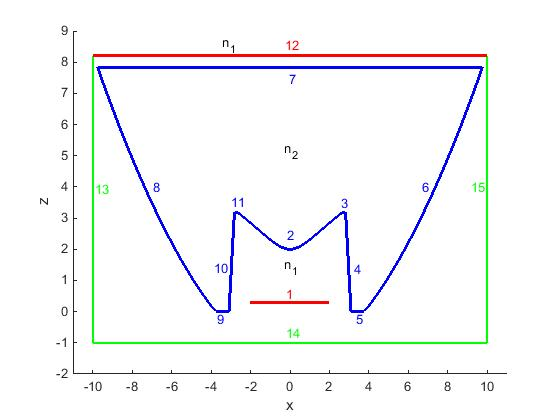
\includegraphics[width=0.7\textwidth]{TIR}
  \end{center}
  \caption{\textbf{Shape of the TIR-collimator.} Each line of the system is labeled with a number.
   The shape of the collimator is shown in blue.
   Three detectors depicted with green lines (surfaces $13$, $14$, and $15$) are located at the left, the right and the bottom of the optical system. The source (line $1$) and the target (line $12$) are depicted in red.}
%The sagitta of the lens is approximately $1.17$.}
  \label{fig:tir}
\end{figure}
\\ \indent
Using PS ray tracing explained in Section \ref{sec:PS_raytracing} with parameters $\varepsilon_{\variabile{q}_1}^{\textrm{max}} = 0.05/4$, $ \varepsilon_{\variabile{p}_1}^\textrm{max} = 0.05/8, $ $\varepsilon_{\variabile{q}_1}^\textrm{min} = 0.8/4$ and $\varepsilon_{\variabile{p}_1}^\textrm{min} = 0.8/8$, around $1.67 \cdot 10^4$ rays are traced (see Table \ref{tab:table}). The ray distribution at the source PS is shown in Figure \ref{fig:sourcePS}, where we depicted the rays that follow the same path with the same color. Seven different paths are found. The yellow rays follow path $\Pi_1 = (1, 2, 7, 12)$;
   the red rays follow path $\Pi_2 ~= ~(1, 4, 6, 7, 12)$; the green rays follow path $\Pi_3 = (1, 10, 8, 7, 12)$;
   the blue rays follow path $\Pi_4= (1, 3, 7, 12)$ and the magenta rays follow path $\Pi_5= (1, 11, 7, 12)$. The rays located inside the white areas correspond to rays that do not reach the target, they follow either path $\Pi_6 = (1, 4, 7, 6, 15)$ or path $\Pi_7 = (1,10,7,8,13)$ and they do not give any contribution to the target intensity.
\begin{figure}[t]
\label{fig:sourcePS}
  \begin{center}
  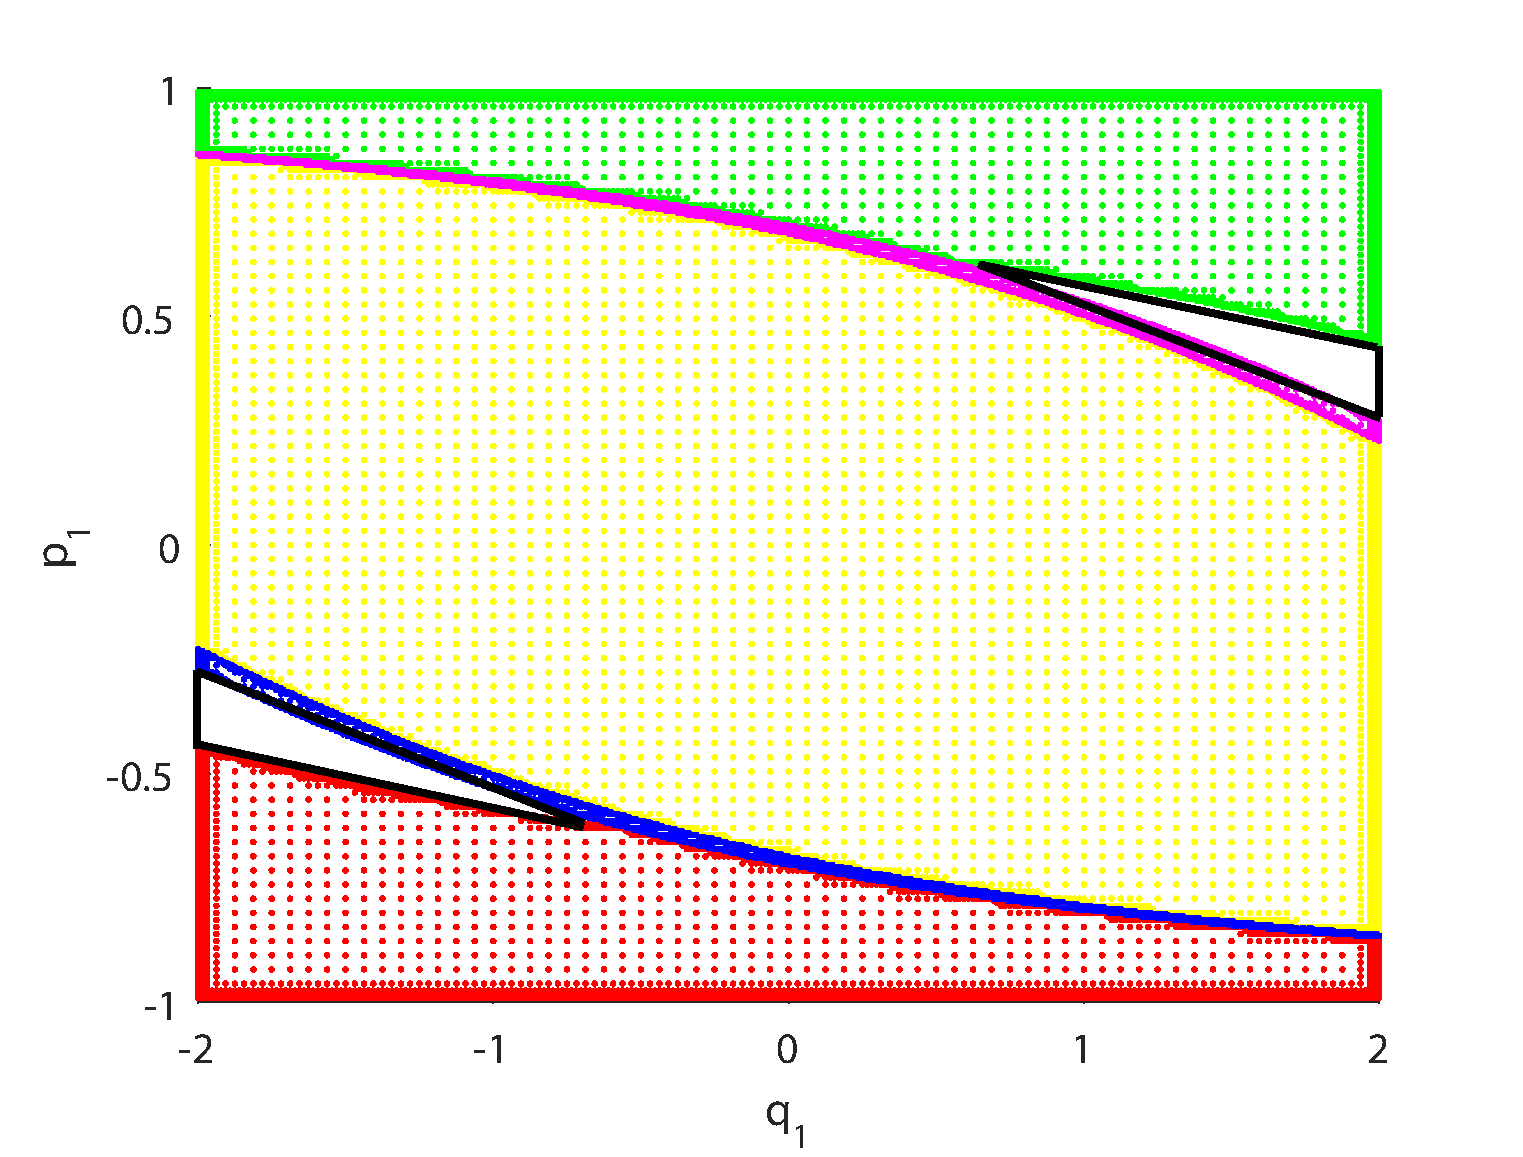
\includegraphics[width=0.8\textwidth]{source1}
  \end{center}
  \caption{\textbf{Distribution of the rays on \point{S}{}{}}. Around $1.67 \cdot 10^4$ rays are traced using the triangulation refinement with parameters:
  $\varepsilon_\variabile{q}^\textrm{max} = 0.8/4 ,$ $ \varepsilon_{\variabile{p}}^\textrm{max} = 0.08/8, $ $\varepsilon_{\variabile{q}}^\textrm{min} = 0.05/4, \varepsilon_\variabile{p}^\textrm{min} = 0.05/8$. Rays that belong to the same region are depicted with the same color. The rays located inside the white areas do not reach the target. The boundaries of the two white regions are approximated by triangles depicted with black lines.}
 \label{fig:sourcePS}
\end{figure}
Note that, given two adjacent paths, the corresponding regions in \set{S}{}{} have usually a common boundary. 
Since for this system not all the rays emitted by the source arrive at the target, $U_{\textrm{t}}$ needs to be compared to the \'{e}tendue $U_1$ at the source given by only those rays that reach the target (the rays that follow paths $\Pi_6$ and 
$\Pi_7$ are discarded). To this purpose $U_1$ is calculated by removing from the total area $U$ of \set{S}{}{} those areas occupied by the regions formed by the rays that hit the left or the right detector (white regions in Figure $\ref{fig:sourcePS}$).  For the TIR collimator in Figure \ref{fig:tir}, $U$ is obtained from (\ref{eq:etenduesource1}), the source \'{e}tendue $U_1$ corresponding to the area covered by the rays that arrive at the target can be approximated by:
 \begin{equation}\label{eq:Usource}
 U_{1} = U-2A_{T},
 \end{equation}
 where $U=8$ and $A_{T}$ is the approximated area of the triangles shown in Figure \ref{fig:sourcePS} with black lines.\\ \indent  Next, $U_{\textrm{t}}$ is calculated several times from (\ref{eq:etenduetarg1}) where every time the boundaries $\partial$\set{R}{}{}$(\Pi)$ are obtained by using $\alpha$-shapes for a different value of $\alpha$. 
%An accurate approximation of $\partial$\set{R}{}{}$(\Pi)$ gives a value of $U_{\textrm{t}}$ close to the exact \'{e}tendue. 
%Matching $U_1$ with all the approximations of $U_{\textrm{t}}$ we find the best value $\alpha_c$ of $\alpha$ that approximates $\partial$\set{R}{}{}$(\Pi)$ and, therefore, $U_{\textrm{t}}$. 
\\ \indent To clarify this concept, in Figure \ref{fig:etendueTS} we provide an example where the source \'{e}tendue $U_1$ and target \'{e}tendue $U_{\textrm{t}}$ are computed from a set of around $1.67\cdot 10^4$ rays. The approximated source \'{e}tendue $U_1\approx 7.77$ is depicted with the red line. The blue line shows how the \'{e}tendue at the target changes as a function of $\alpha$. The smallest difference $\Delta U = |U_1-U_{\textrm{t}}|$ is obtained using $\alpha = \alpha_\textrm{c} = 0.08$.
 \begin{figure}[t]
  \begin{center}
  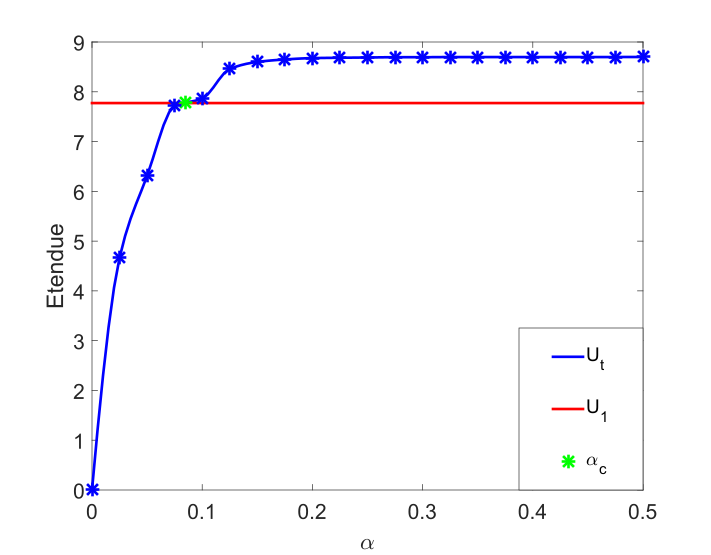
\includegraphics[width=0.7 \textwidth]{etendue_alpha_shapes}
  \end{center}
  \caption{\textbf{Etendue for the TIR-collimator.} $U_\textrm{t}$ is computed for a range of values for $\alpha$. $U_1 \approx 7.77$
   The green dot indicates the value of $\alpha_\textrm{c} = 0.08$ which gives a good approximation of the boundaries $\partial$\set{R}{}{}$(\Pi)$ at the target.
   Around $1.67 \cdot 10^4$ rays have been traced using PS ray tracing.
  }
  \label{fig:etendueTS}
\end{figure}
In Figure \ref{fig:targetPS} we show the boundaries 
$\partial$\set{R}{}{}$(\Pi)$ in target PS with $\alpha_\textrm{c}=0.08$ and tracing $1.67\cdot10^4$ rays.
  \begin{figure}[h]
  \begin{center}
  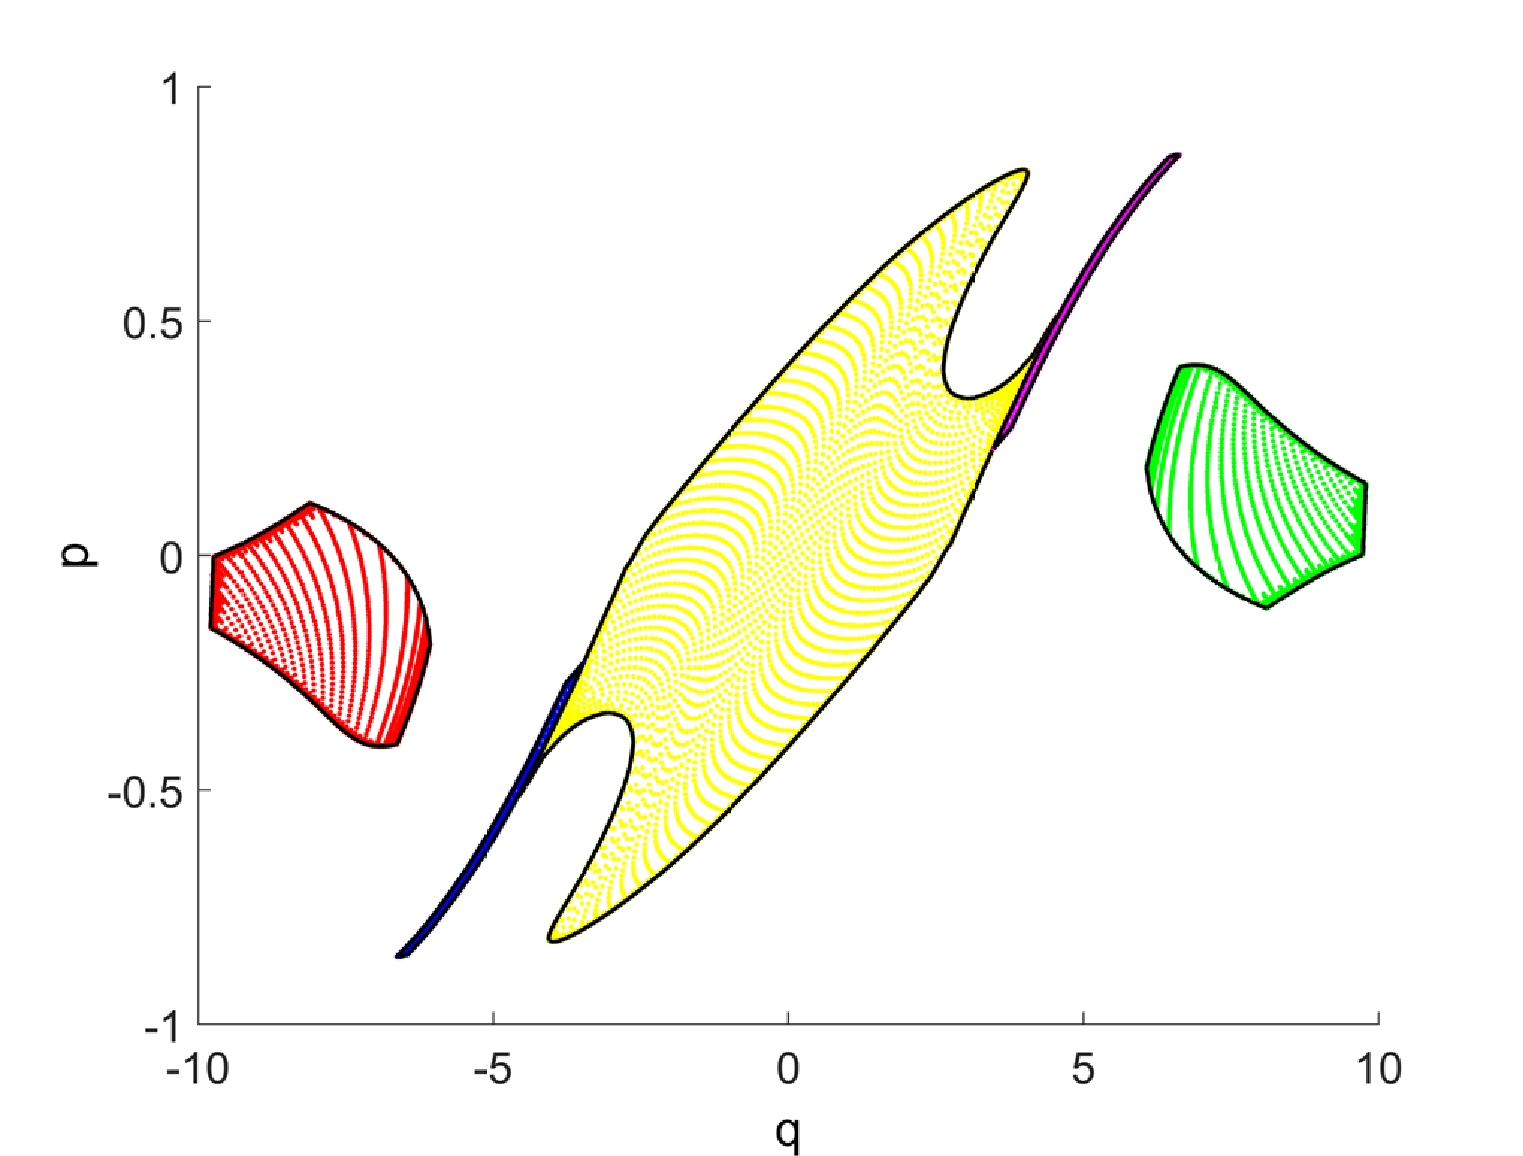
\includegraphics[width=0.7\textwidth]{target_alpha_shapes}
  \end{center}
  \caption{\textbf{Target PS representation.} A set of $1.67 \cdot 10^4$ rays are traced.
  Rays that follow the same path are depicted with the same color. The choice of the colors is consistent with Figure $\ref{fig:sourcePS}$. The boundaries $\partial$\set{R}{}{}$(\Pi)$ are computed through the $\alpha$-shapes method with $\alpha = \alpha_\textrm{c} = 0.08$.}
  \label{fig:targetPS}
\end{figure}
The target intensity $I_{\textrm{PS}}(\variabile{p})$ for $\variabile{p}\in[-1,1]$ is obtained from Equation (\ref{eta2}). \\ \indent
To validate our method we compare the PS intensity with the QMC intensity. 
To this purpose a partitioning $P_2:-1=\variabile{p}_{0}<\variabile{p}_1<\cdots<\variabile{p}_{\nbin}=1$ of the interval $[-1,1]$ into $\nbin=100$ bins is considered. 
The averaged and normalized PS intensity $\hat{I}_{\textrm{PS}}$ is calculated for every 
$\big(\variabile{p}^{\variabile{h}+1/2} = \frac{1}{2}(\variabile{p}^{\variabile{h}+1}+ \variabile{p}^{\variabile{h}})\big)_{\variabile{h}=0, \cdots, \nbin-1}$ dividing the PS averaged intensity by the total \'{e}tendue:
\begin{equation}\label{eq:normalized_PS_intensity}
\hat{I}_{\textrm{PS}}(\variabile{p}^{\variabile{h}+1/2}) = \frac{1}{U_{\textrm{t}}}\int_{\variabile{p}_{\variabile{h}}}^{\variabile{p}_{\variabile{h}+1}} I_{\textrm{PS}}(\variabile{p})\textrm{d}\variabile{p}.
\end{equation}
The averaged and normalized QMC intensity $\big(\hat{I}_{\textrm{QMC}}(\variabile{p}^{\variabile{h}+1/2})\big)_{\variabile{h} = 0, \cdots, \nbin-1}$ is given by
\begin{equation}\label{eq:normalized_MC_intensity}
\hat{I}_{\textrm{QMC}}(\variabile{p}^{\variabile{h}+1/2}) = \frac{\nrays[\variabile{p}^{\variabile{h}},\variabile{p}^{\variabile{h}+1})}{\nrays[-1,1)} 
\qquad \mbox{ for } \variabile{p}\in[\variabile{p}^{\variabile{h}}, \variabile{p}^{\variabile{h}+1}).
\end{equation} 
Both approximate intensities $\hat{I}_{\textrm{A}} (\textrm{A} = \textrm{PS}, \textrm{QMC})$ are compared to an intensity $\hat{I}_{\textrm{ref}}$ taken as a reference. 

For some optical systems, there is an explicit solution for the target intensity but this is not the case of the TIR-collimator.
Therefore, a QMC simulation with $10^7$ rays is used to obtain the averaged normalized intensity $\hat{I}_{\textrm{ref}}$.
The intensity profile $\hat{I}_{\textrm{PS}}
$ obtained using PS ray tracing with $8.3\cdot 10^4$ rays and $\alpha= \alpha_\textrm{c} = 0.06$ is depicted in Figure \ref{fig:intensityMCPS} with a red line.
$\hat{I}_{\textrm{PS}}$ is hardly distinguishable from $\hat{I}_{\textrm{ref}}$ which is indicated with the dashed and blue line in Figure $\ref{fig:intensityMCPS}$.\\ \indent
  \begin{figure}[h]
    \centering
    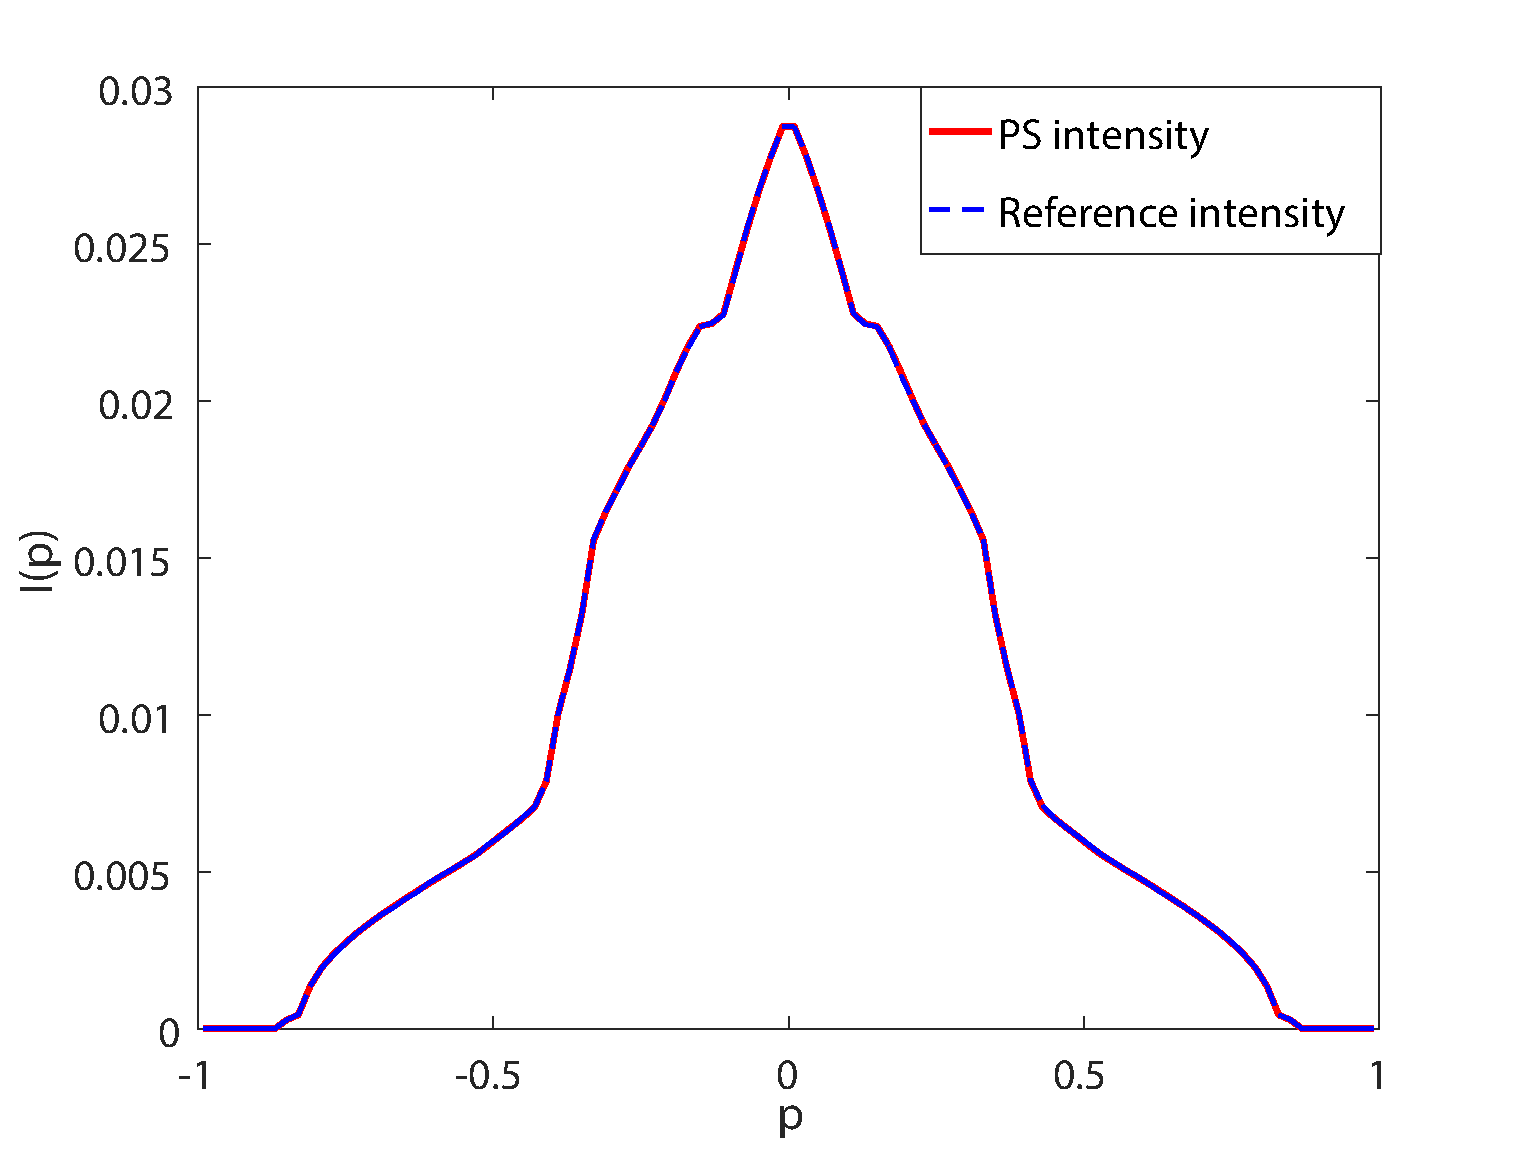
\includegraphics[width=0.7\textwidth]{intensity_alpha_shapes}
\caption{\textbf{Target intensity profile.}
The exact intensity is computed using the QMC method for a set of $10^7$ rays. For the PS intensity a set of $6.3\cdot 10^4$
rays is considered and $\alpha_\textrm{c} = 0.06$ is chosen to compute the boundaries $\partial$\set{R}{}{}$(\Pi)$.}
  \label{fig:intensityMCPS}
\end{figure}
Finally, we calculate the error between $\hat{I}_{\textrm{A}}$ and $\hat{I}_{\textrm{ref}}$, defined as:
\begin{equation}\label{eq:error}
\mbox{error} = \frac{\sum_{\variabile{h}= 1}^{\nbin}| \hat{I}_{\textrm{A}}(\variabile{p}^{\variabile{h}+1/2}) - \hat{I}_{\textrm{ref}}(\variabile{p}^{\variabile{h}+1/2})|}{\nbin}.
\end{equation}
The QMC and PS intensities are calculated several times increasing the number of rays to improve the accuracy.
Table \ref{tab:table} and \ref{tab:table2} describe how the number of rays traced affects the error. 
In Table \ref{tab:table} the correlation between $\alpha_\textrm{c}$ and the number of rays is evident.
%determined by the values of $\varepsilon^{\textrm{min}}_\variabile{p}$, $\varepsilon^{\textrm{min}}_{\variabile{q}}$, 
%$\varepsilon^{\textrm{max}}_{\variabile{p}}$ and $\varepsilon^{\textrm{max}}_{\variabile{q}}$. 
Note that increasing the number of rays the value of $\alpha_\textrm{c}$ and the corresponding error decrease. 
\begin{table}[htbp] \label{tab:table}
\centering
\caption{\bf Errors of the PS intensity}
\begin{tabular}{lllllll}
 \hline  Number \\ of rays\;  & $\varepsilon^{\textrm{max}}_{\variabile{q}} $  & $\varepsilon^{\textrm{min}}_{\variabile{q}} $   \;     & $\varepsilon^{\textrm{max}}_{\variabile{p}}$\;
  & $\varepsilon^{\textrm{min}}_\variabile{p}$\; & $\alpha_\textrm{c}$  & PS error \\
  \hline 
 $3\,339$ & $0.8$  & $0.05$  & $0.8/2$  & $0.05/2$ & $0.14$ & $1.47\cdot10^{-3}$ \\
$7\,567$  & $0.8/2$  & $0.05/2$  & $0.8/4$  & $0.05/4$ & $0.10$ & $3.01\cdot 10^{-4}$  \\
$16\,755$  & $0.8/4$  & $0.05/4$  & $0.8/8$  & $0.05/8$ & $0.08$ & $8.60\cdot 10^{-5}$ \\
 $83\,005$ & $0.8/16$  & $0.05/16$  & $0.8/32$  & $0.05/32$ & $0.06$ & $1.31\cdot 10^{-5}$ \\
 \hline
 \end{tabular}
 \label{tab:table}
 \end{table}
\\ \indent In Table \ref{tab:table2} the numerical results of QMC ray tracing are reported.
Increasing the number of rays traced, the error gradually decreases.
\begin{table}[htbp]
\centering
\caption{\bf Error of the QMC intensity}
\begin{tabular}{ll} \hline   Number of rays\; & QMC error\\
 \hline $10^3$  & $1.65\cdot10^{-3}$ \\
$10^4$  & $3.96\cdot 10^{-4}$  \\
 $10^5$  & $6.36\cdot 10^{-4}$ \\ 
$10^6$  & $1.02\cdot 10^{-5}$ \\
 \hline
 \end{tabular}
 \label{tab:table2}
 \end{table}
\noindent In Figure $\ref{fig:error}$, the results listed in Table $\ref{tab:table}$ and Table $\ref{tab:table2}$ are shown. The red line depicts the convergence of the PS error and the blue line indicates the QMC error.
\begin{figure}[t]
  \begin{center}
  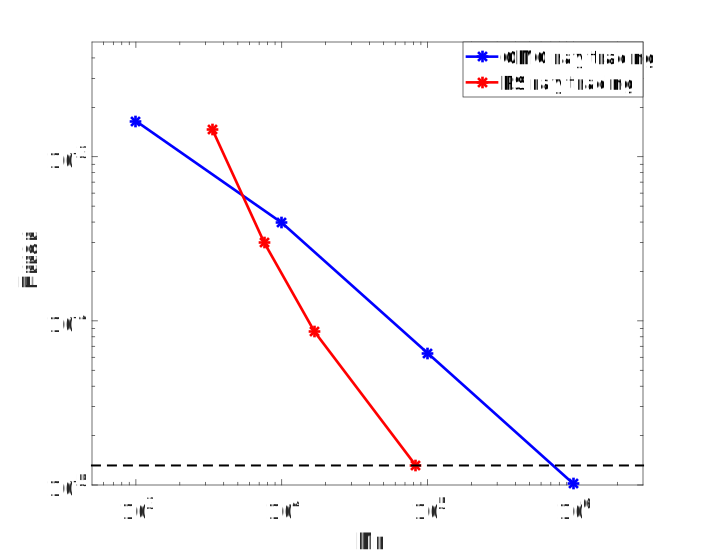
\includegraphics[width=0.7\textwidth]{error_alpha_shapes_vs_qmc_curved}
  \end{center}
  \caption{\textbf{PS and QMC errors as a function of the number of rays}
  The horizontal dotted line shows that an error equal to $1.31\cdot  10^{-5}$ can be obtained tracing almost $10$ times fewer rays in phase space.}
  \label{fig:error}
\end{figure}
%Note from Figure \ref{fig:error} that the error for the QMC method decreases as $\frac{1}{\sqrt{\nrays}}$, while for the PS simulation the speed of convergence is much higher.\\ \indent
We need to emphasize that the convergence of the error of PS ray tracing for increasing $\nrays$ may change according to the design of the optical system.
This is because the approximation of the boundaries in PS depends on the accuracy of the $\alpha$-shapes method.
The $\alpha$-shapes procedure is unable to properly detect the boundaries of regions with a sharp turn if not enough points are given
\cite{teichmann1998surface}. Indeed, on the one hand a low density requires a large value of $\alpha$ to accept the triangles in a region, on the other hand,
 choosing $\alpha$ too large, the shape of the region could be destroyed. Indeed, increasing $\alpha$ more triangles are kept and triangles inside the regions \set{R}{}{}$(\Pi)$ could be taken into account creating holes in \set{R}{}{}$(\Pi)$.
\begin{figure}[h]
\centering
\begin{subfigure}{.48\textwidth}
  \centering
  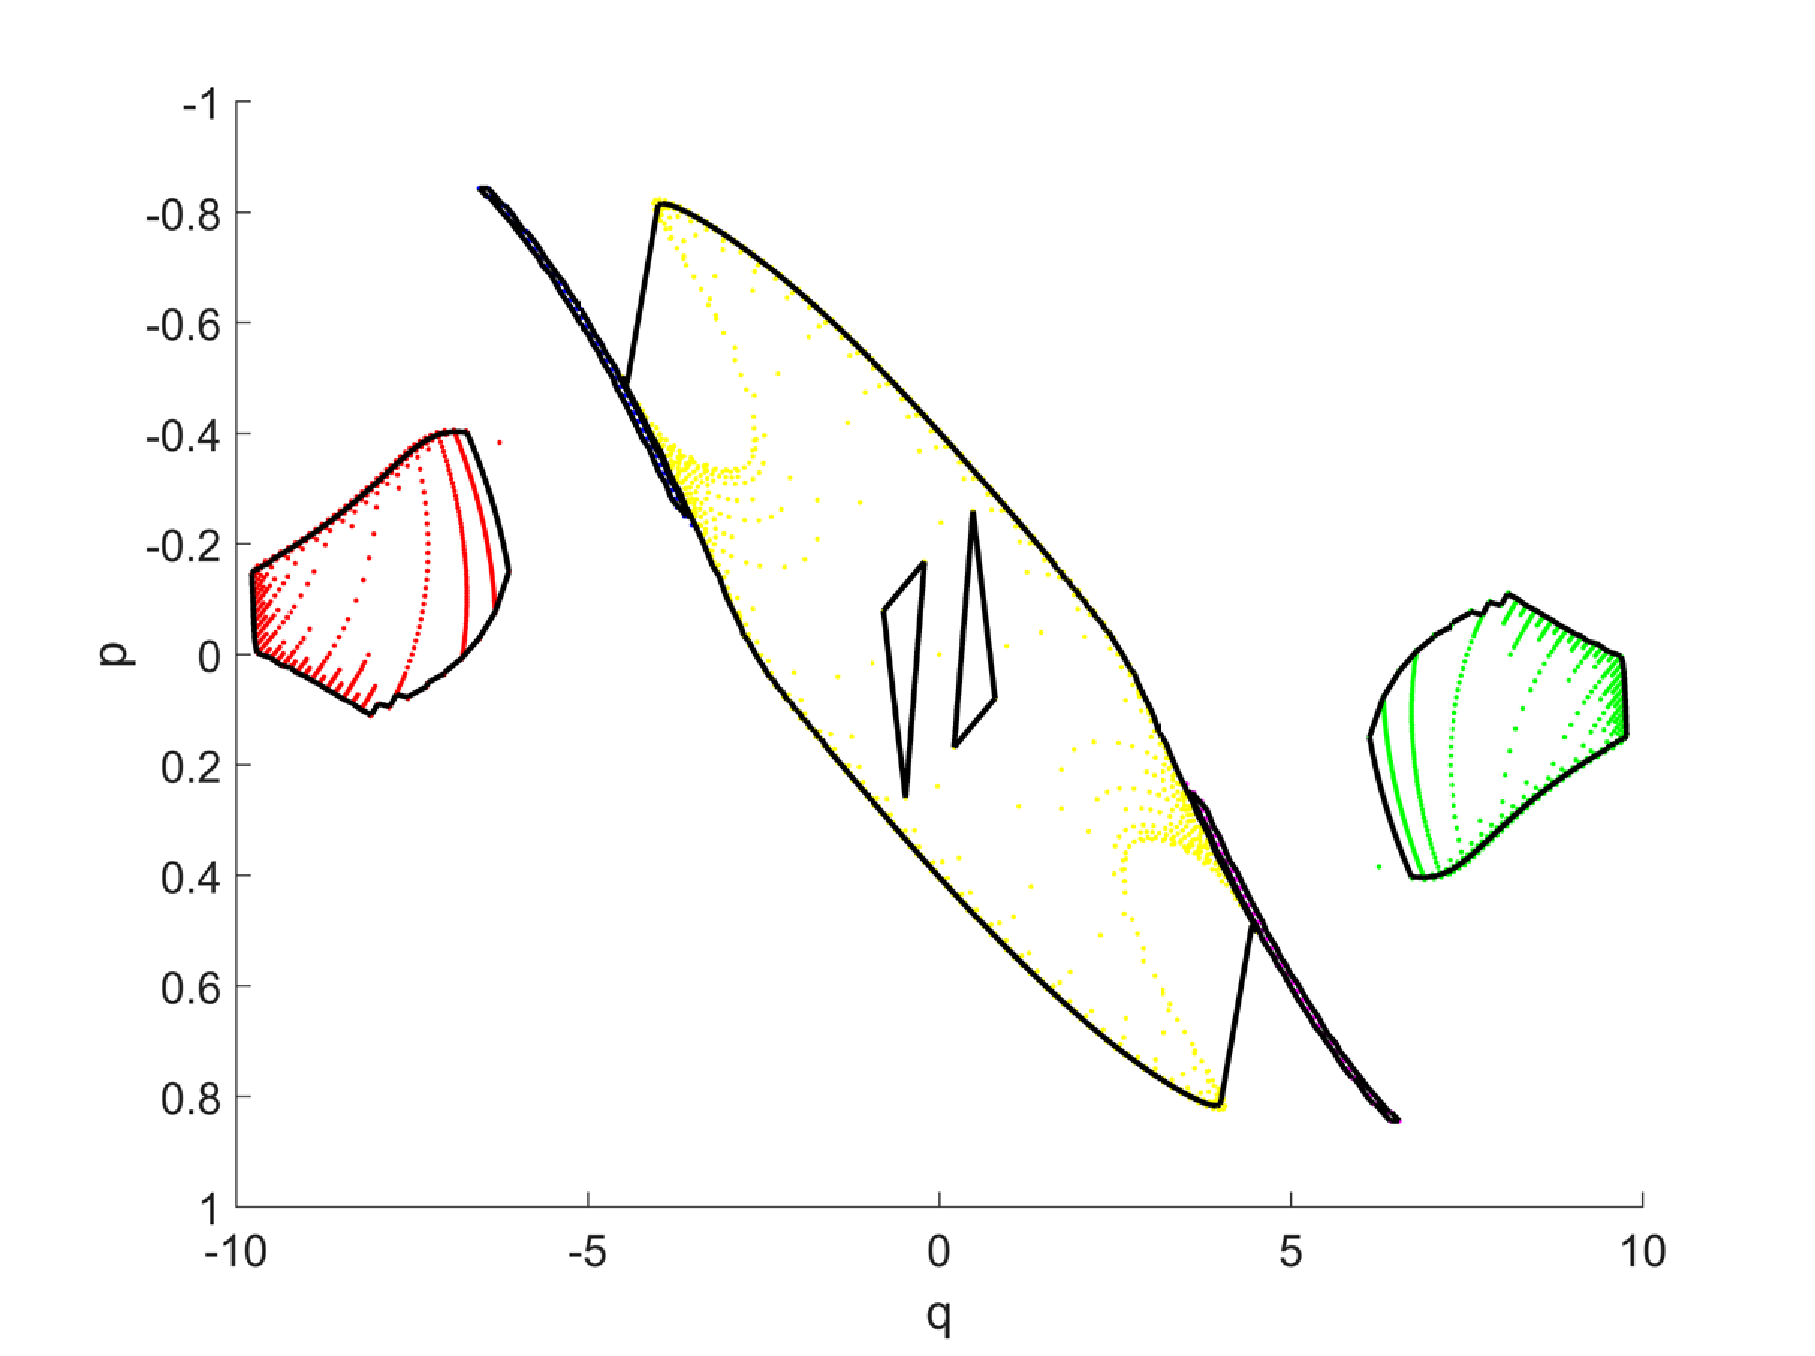
\includegraphics[width=\textwidth]{boundaries_alpha1}
  \caption{Boundaries approximation obtained using the $\alpha$-shapes method with $\alpha_\textrm{c} = 0.3$ (black lines).}
\end{subfigure}
\hfill
\begin{subfigure}{.48\textwidth}
  \centering
  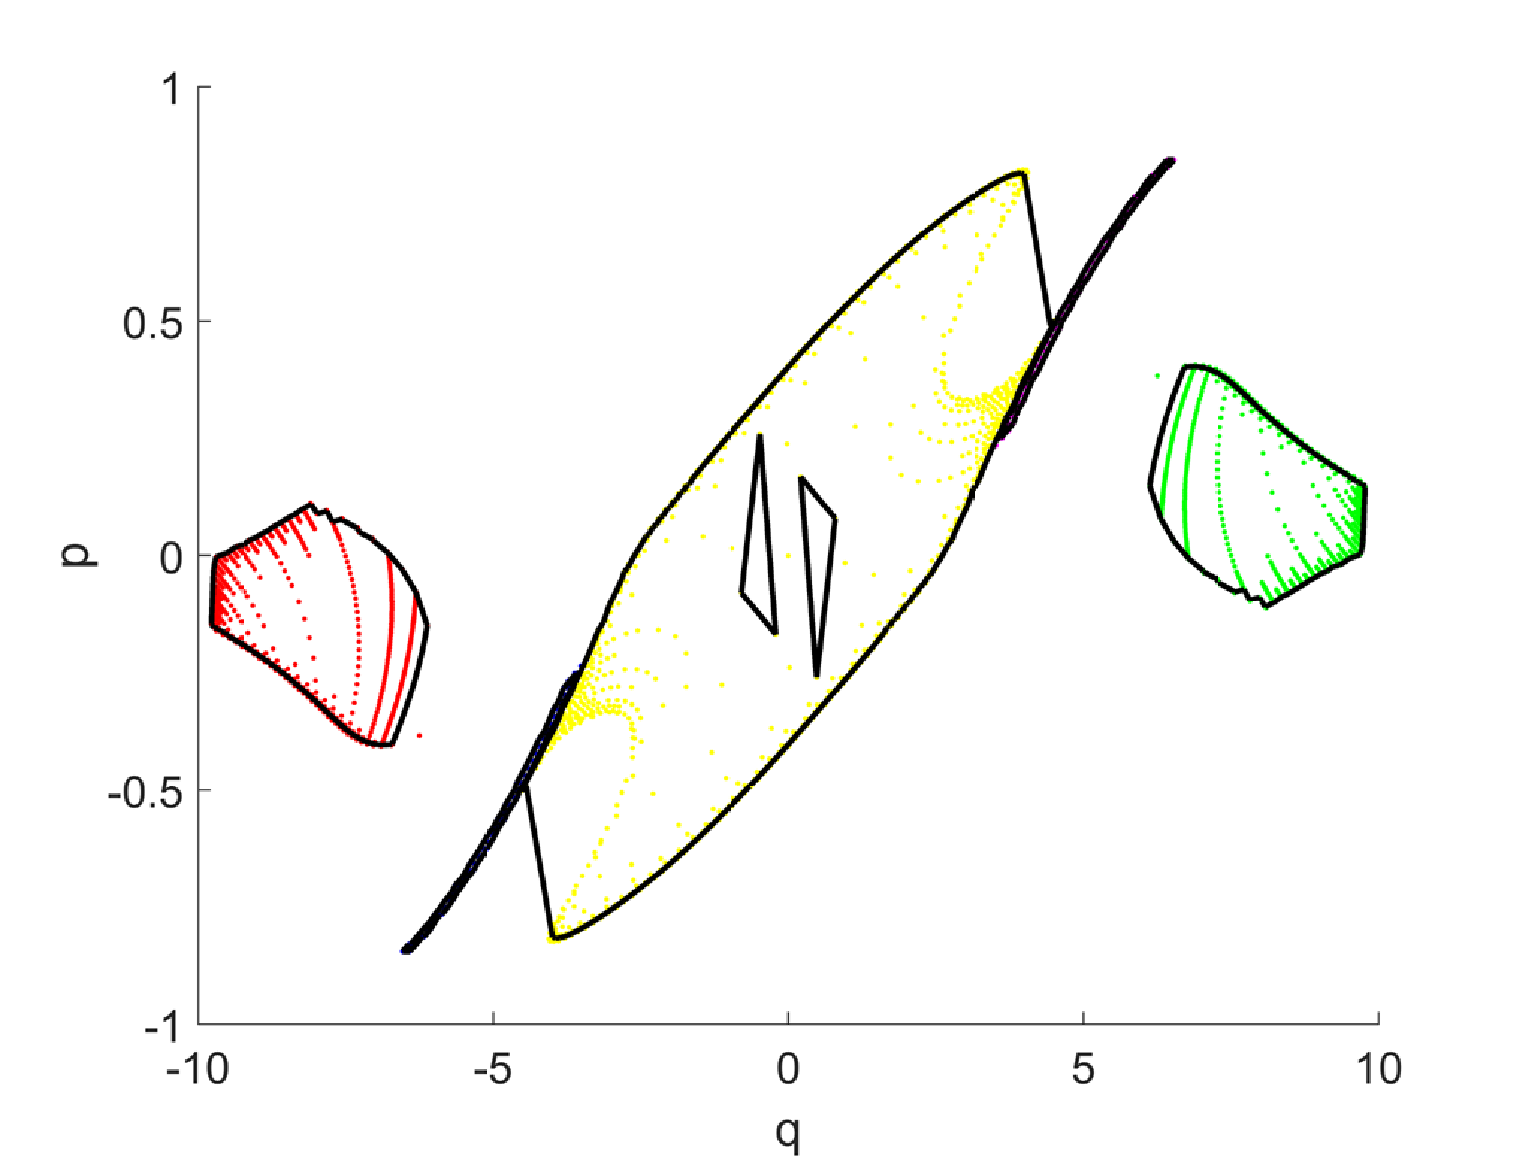
\includegraphics[width=\textwidth]{boundaries_alpha2}
  \caption{Boundaries approximation obtained using the $\alpha$-shapes method with $\alpha_\textrm{c} = 0.31$ (black lines).}
\end{subfigure}
\caption{\textbf{Approximated boundaries at the target PS.} Tracing $3339$ rays and using $\alpha$-shapes, the boundaries cannot be approximated well. 
A small change of the parameter $\alpha$ leads to a completely different approximation of the boundaries.}
\label{fig:Tir1}
\end{figure}
Figure $\ref{fig:Tir1}$ clarifies this concept showing that the region formed by rays that hit the lens is hard to approximate when there is a small number of rays inside the region. Consequently either a region bigger than the area covered by the rays is obtained or some triangles which are not part of the boundaries are included in the triangulation. This results in an inaccurate intensity (either too high or to low). To obtain a good approximation of the boundaries of these kind of patches more rays have to be traced. The PS error decreases very fast increasing the number of rays (see Table
 \ref{tab:table} and Figure \ref{fig:error}).
 \\\indent To show how the error plot changes according to the regularity of the shape of the regions $\partial$\set{R}{}{}$(\Pi)$, we consider another example of a TIR-collimator.
 Figure $\ref{fig:Tir1}$ shows that the hardest region to approximate is given by those rays that follow path $\Pi_1 ~=~ (1,2,7,12)$.
 We therefore consider a TIR-collimator with a flatter lens and with the target located at a smaller distance to the top (see Figure $\ref{fig:analyticlens}$). 
The source $\point{S}= [-2,2]$ (surface number $1$) is located in air at a height $\variabile{z}_1 = 0.3$ from the $x$-axis.
       The target $\point{T}= [-9.7, 9.7]$ (surface $12$) is parallel to the source and is located in air at a height $ \variabile{z}= 7.85$.
       The shape of the collimator is shown as a blue line.
       Three detectors depicted with green lines (surfaces $13$, $14$, and $15$) are located at the left, the right and the bottom of the optical system.
 \\ \indent Tracing around $3\cdot10^3$ rays using PS ray tracing, we obtain the target rays distribution shown in Figure $\ref{fig:Tir2}$. 
Compared with the distribution in Figure \ref{fig:targetPS}, we note that the extremities at top and bottom of the region formed by the rays that hit the lens are less pronounced.
Moreover a target located very close to the top makes the shape of that region less stretched along the $\variabile{q}$-axis.
Therefore, it is expected that the $\alpha$-shapes method performs better for a small number of rays.
\begin{figure}[h]
  \begin{center}
  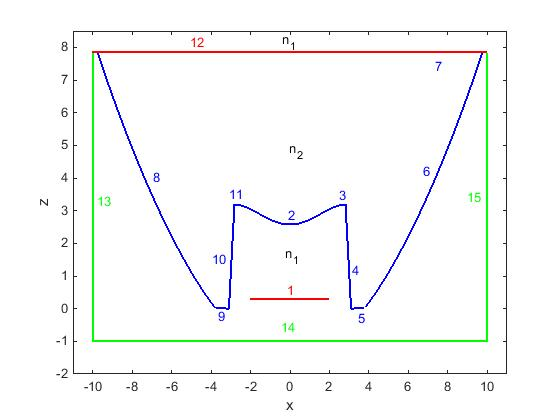
\includegraphics[width=0.7\textwidth]{tir_analytic2}
   \end{center}
    \caption{\textbf{Shape of the TIR-collimator.} Each line of the system is labeled with a number.
       $n_1 = 1$ is the refraction index of the medium (air) where the source and the target are located, and
       $n_2 = 1.5 $ the refraction index of the medium (glass) inside the optical system.} 
%The sagitta of the lens is equal to $0.6$.}
 \label{fig:analyticlens}
\end{figure}
 \begin{figure}[h]
  \begin{center}
       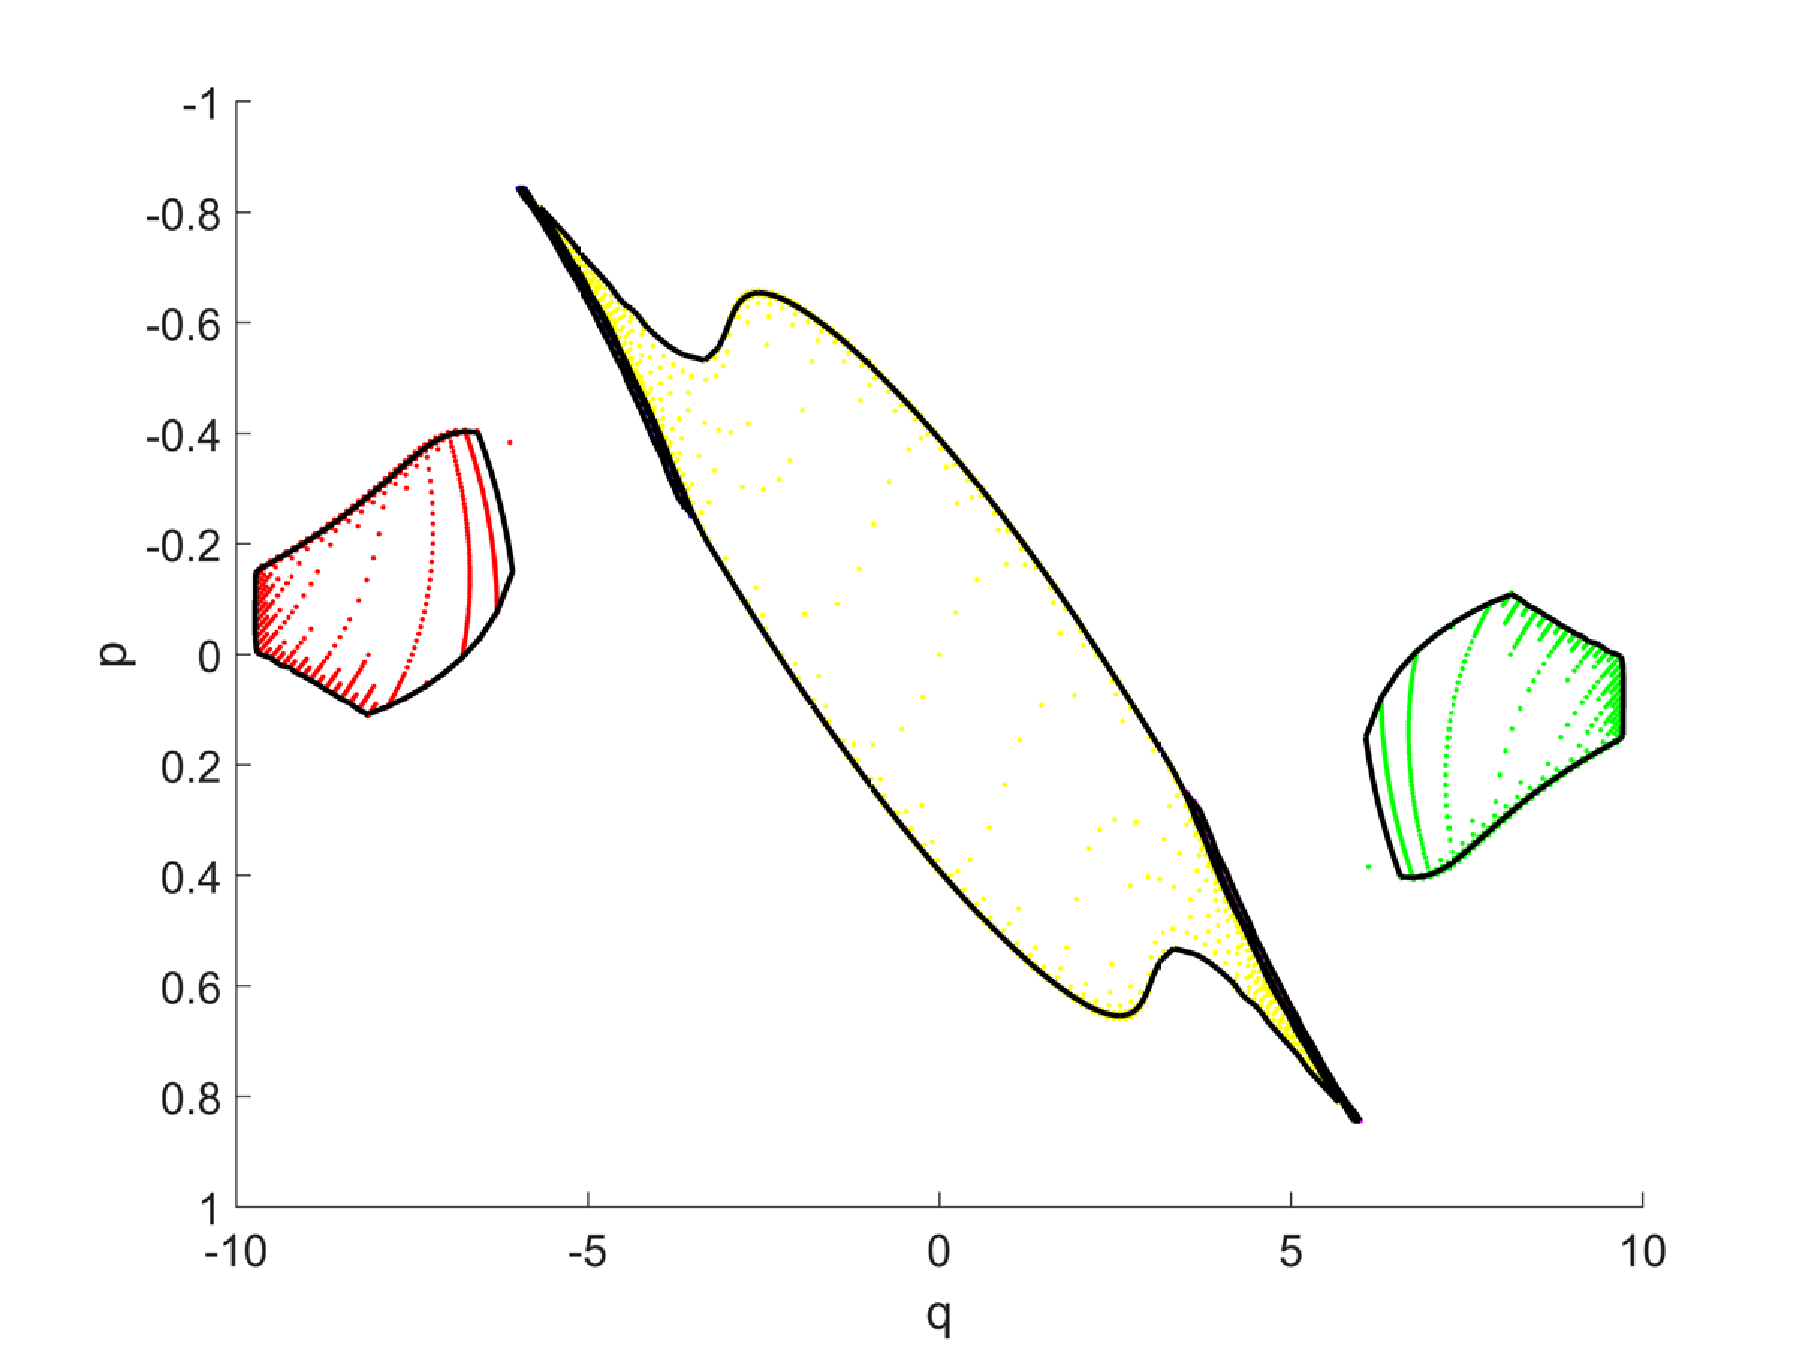
\includegraphics[width=0.7\textwidth]{boundaries_alpha3}
   \end{center}
        \caption{\textbf{Target phase space for the TIR-collimator depicted in
        Figure \ref{fig:analyticlens}.} The black line depicts the best approximation of $\partial$\set{R}{}{}$(\Pi)$ for $3\cdot 10^3$ rays. 
The $\alpha$-shapes method gives an accurate approximation of the boundaries for $\alpha_\textrm{c} = 0.9$.}
  \label{fig:Tir2}
\end{figure}
\\ \indent PS and QMC ray tracing are implemented for the TIR-collimator in Figure \ref{fig:analyticlens}. The approximated intensities $\hat{I}_{\textrm{A}}$ $(\textrm{A} = \textrm{PS}, \textrm{QMC})$ are compared to the reference intensity $\hat{I}_{\textrm{ref}}$ (QMC ray tracing with $10^7$ rays).
PS error is depicted with the red line and, QMC error is depicted with the blue line. \\ \indent
% Lets indicate with $\big(\hat{I}_{\textrm{A}, n}\big)_{n \in \mathbb{N}}$ the sequence of the approximated intensity. Every term of the sequence is calculated by increasing the number of rays, for example $\hat{I}_{\textrm{A}, 1}$ is computed tracing $\nrays = 10$ rays,   $\hat{I}_{\textrm{A}, 2}$ is computed tracing $\nrays = 100$ rays, and so on. The speed or rate of convergence of the approximate intensity $\big(\hat{I}_{\textrm{A}, n}\big)$ describes how quickly the terms of sequence $\big(\hat{I}_{\textrm{A}, n}\big)$ converge to the reference intensity $\hat{I}_{\textrm{ref}}$ by increasing the number of rays. Suppose $m$ is a real number, the sequence $\big(\hat{I}_{\textrm{A}, n}\big)$ converges to $\hat{I}_{\textrm{ref}}$ if
%\begin{equation}
%\lim_{\nrays\rightarrow \infty} \frac{|\hat{I}_{\textrm{A}, n+1}-\hat{I}_{\textrm{ref}}|}{|\hat{I}_{\textrm{A}, n}-\hat{I}_{\textrm{ref}}|^m} = \mu
%\end{equation}
%and $\mu$ is called the rate of convergence and $m$ is the order of convergence. For $m\in[0,1]$ we have the linear convergence, for $m=2$ the quadratic convergence, etc. 
%\\ \indent
Numerical results show that, for the TIR-collimator in Figure \ref{fig:analyticlens}, the computational time needed to achieve an error of the order of $10^{-5}$ is reduced using PS ray tracing compared with QMC ray tracing.
\begin{figure}[t]
 \begin{center}
   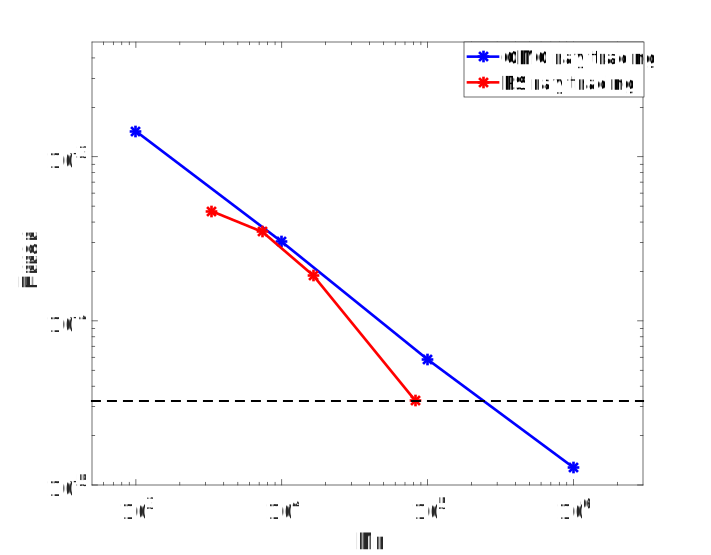
\includegraphics[width=\textwidth]{error_alpha_shapes_vs_qmc_flat}
    \end{center}
     \caption{\textbf{PS and QMC errors.}}
%The red line depicts the error using the $\alpha$-shapes method to compute the boundaries. 
%The blue line shows the error between the Monte Carlo intensity and the exact intensity.
%     The dashed black line represents a straight line with slope $-\frac{1}{2}$.
%   The dashed blue line represents a straight line with slope $-1$.}
 \label{fig:error2}
\end{figure}
\section{Conclusion}
The aim of this chapter was using $\alpha$-shapes to detect the boundaries of the regions formed by the rays traced.\\
\indent First, we reported some theory about $\alpha$-shapes which are commonly used to approximate the shape formed by a point cloud. 
These methods depend on a parameter $\alpha$ that in most cases can be determined only by simulations. 
\\ \indent Using \'{e}tendue conservation, we developed a new approach to detect the value of $\alpha$ that better approximates the boundaries in target PS. 
We applied $\alpha$-shapes to two different kind of TIR-collimators. The target PS intensity was computed for both systems several times increasing every time the number of rays traced. Finally, the corresponding errors between the approximated intensities and a reference intensity was calculated. We observed that PS ray tracing allows tracing far less rays compared to QMC ray tracing. Numerical results show that using PS ray tracing the desired accuracy can be achieved reducing significantly the number of rays traced.\\ \indent 
However, we observed that the error convergence for PS ray tracing strongly depends on the design of the optical system (shapes of the region in target PS). Indeed, the accuracy of the intensity is related to the precision of the $\alpha$-shape, that is, to the choice of the parameter value of $\alpha$. For more complicated shapes in PS, more rays need to be traced for a good boundaries reconstruction.\\ \indent
In order to remove the dependence of PS ray tracing on the parameter $\alpha$, we will construct another procedure to detect the boundaries of the regions in target PS. 
The new technique is based on the triangulation refinement explained in Section \ref{sec:PS_raytracing}. The details are explained in the next chapter and numerical results are reported for several optical systems. 











































